%%%%%%%%%%%%%%%%%%%%%%%%%%%%%%%%%%%%%%%%%
% Beamer Presentation
% LaTeX Template
% Version 1.0 (10/11/12)
%
% This template has been downloaded from:
% http://www.LaTeXTemplates.com
%
% License:
% CC BY-NC-SA 3.0 (http://creativecommons.org/licenses/by-nc-sa/3.0/)
%
%%%%%%%%%%%%%%%%%%%%%%%%%%%%%%%%%%%%%%%%%

%----------------------------------------------------------------------------------------
%	PACKAGES AND THEMES
%----------------------------------------------------------------------------------------

\documentclass{beamer}

\mode<presentation> {

% The Beamer class comes with a number of default slide themes
% which change the colors and layouts of slides. Below this is a list
% of all the themes, uncomment each in turn to see what they look like.

%\usetheme{default}
%\usetheme{AnnArbor}
%\usetheme{Antibes}
%\usetheme{Bergen}
%\usetheme{Berkeley}
%\usetheme{Berlin}
%\usetheme{Boadilla}
%\usetheme{CambridgeUS}
%\usetheme{Copenhagen}
%\usetheme{Darmstadt}
%\usetheme{Dresden}
%\usetheme{Frankfurt}
%\usetheme{Goettingen}
%\usetheme{Hannover}
%\usetheme{Ilmenau}
%\usetheme{JuanLesPins}
%\usetheme{Luebeck}
\usetheme{Madrid}
%\usetheme{Malmoe}
%\usetheme{Marburg}
%\usetheme{Montpellier}
%\usetheme{PaloAlto}
%\usetheme{Pittsburgh}
%\usetheme{Rochester}
%\usetheme{Singapore}
%\usetheme{Szeged}
%\usetheme{Warsaw}

% As well as themes, the Beamer class has a number of color themes
% for any slide theme. Uncomment each of these in turn to see how it
% changes the colors of your current slide theme.

%\usecolortheme{albatross}
%\usecolortheme{beaver}
%\usecolortheme{beetle}
%\usecolortheme{crane}
%\usecolortheme{dolphin}
%\usecolortheme{dove}
%\usecolortheme{fly}
%\usecolortheme{lily}
%\usecolortheme{orchid}
%\usecolortheme{rose}
%\usecolortheme{seagull}
%\usecolortheme{seahorse}
%\usecolortheme{whale}
%\usecolortheme{wolverine}

%\setbeamertemplate{footline} % To remove the footer line in all slides uncomment this line
%\setbeamertemplate{footline}[page number] % To replace the footer line in all slides with a simple slide count uncomment this line

%\setbeamertemplate{navigation symbols}{} % To remove the navigation symbols from the bottom of all slides uncomment this line
}

\usepackage{graphicx} % Allows including images
\usepackage{booktabs} % Allows the use of \toprule, \midrule and \bottomrule in tables
\usepackage{svg}
\usepackage{amsmath}
\usepackage{color}
\usepackage{animate}
\usepackage{amssymb}

\newcommand{\MR}[1]{{\bf \color{blue} [MR: #1]}}

%----------------------------------------------------------------------------------------
%	TITLE PAGE
%----------------------------------------------------------------------------------------

\title[Distributed MST]{A Simple Deterministic Distributed MST Algorithm, with Near-Optimal Time and Message Complexities} % The short title appears at the bottom of every slide, the full title is only on the title page

\author{Mengye Ren} % Your name
\institute[Univ. of Toronto] % Your institution as it will appear on the bottom of every slide, may be shorthand to save space
{
University of Toronto \\ % Your institution for the title page
\textit{mren@cs.toronto.edu} % Your email address
\\
\medskip
Paper by Michael Elkin\\
Department of Computer Science\\
Ben-Gurion University of The Negev, Beer-Sheva, Israel\\
\medskip
}
\date{\today} % Date, can be changed to a custom date

\begin{document}

\begin{frame}
\titlepage % Print the title page as the first slide
\end{frame}

\begin{frame}
\frametitle{Overview} % Table of contents slide, comment this block out to remove it
\tableofcontents % Throughout your presentation, if you choose to use \section{} and \subsection{} commands, these will automatically be printed on this slide as an overview of your presentation
\end{frame}

%----------------------------------------------------------------------------------------
%	PRESENTATION SLIDES
%----------------------------------------------------------------------------------------
% !TEX root=../presentation_1.tex
\section{Introduction}

\subsection{Minimum-Weight Spanning Tree (MST)}

\begin{frame}
\frametitle{Minimum-Weight Spanning Tree (MST)}

\begin{itemize}
  \item A \textbf{weighted} graph $G = (V,E,W)$. $V$ is a set of vertices and $E$ is a set of edges, and each edge has an associated weight.
  \item A \textbf{spanning tree} is a tree that covers all vertices.
  \item A spanning tree is \textbf{minimum} if the sum of all weights in the tree is the minimum among all spanning trees.
\end{itemize}
\begin{figure}
    \centering
    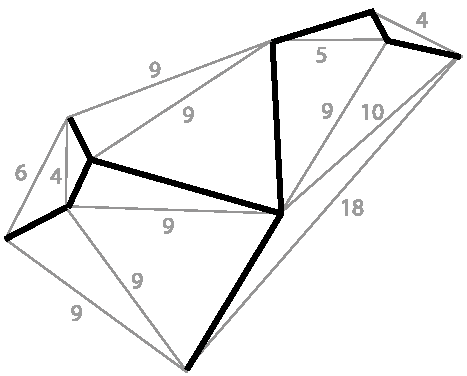
\includegraphics[width=0.4\textwidth]{figures/mst.pdf}
    \caption{An example of MST}
\end{figure}
\end{frame}

\subsection{Practical Applications}

\begin{frame}
\frametitle{Practical Applications}
\begin{itemize}
  \item Building highways.
  \item Building network links.
  \item Broadcasting.
  \item Circuit design.
  \item Clustering, image segmentation.
\end{itemize}
\begin{figure}
    \centering
    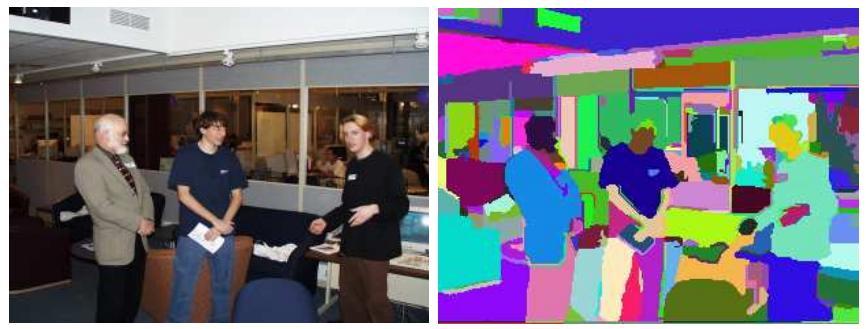
\includegraphics[width=0.6\textwidth]{figures/segmentation.png}
    \caption{An MST-based Image Segmentation Method [FH04]}
\end{figure}
\end{frame}

\subsection{Greedy Sequential Algorithms}

\begin{frame}
\frametitle{Greedy Sequential Algorithms}

\begin{itemize}
\item \textcolor{red}{\textbf{Red}} rule. Let $C$ be a cycle with no red arcs. Select an uncolored arc of $C$ of max weight and color it red. 
\item \textcolor{blue}{\textbf{Blue}} rule. Let $D$ be a cut with no blue arcs. Select an uncolored arc in $D$ of min weight and color it blue.
\end{itemize}
\begin{itemize}
  \item Boruvka's algorithm
    \begin{itemize}
      \item The first MST algorithm developed in the 20s.
      \item Iteratively merging MST forest.
    \end{itemize}
  \item Kruskal's algorithm
    \begin{itemize} 
      \item Iteratively adding minimum weighted edge without forming a cycle.
    \end{itemize}
  \item Prim's algorithm
    \begin{itemize} 
      \item Iteratively expanding the vertices by selecting the minimum weighted outgoing edge.
    \end{itemize}
\end{itemize}
\end{frame}


\begin{frame}
\animategraphics{12}{figures/KruskalDemo-}{0}{9}
\end{frame}
% !TEX root=../presentation_1.tex
\section{Background}

\subsection{Synchronous CONGEST model}

\subsection{Pipeline-MST}

\subsection{GHS [GHS86]}

\subsection{Cole-Vishkin [CV86]}

\subsection{Controlled-GHS [GKP98, KP98]}
% !TEX root=../presentation_1.tex
\section{Method}

\begin{frame}
\frametitle{A Simple Deterministic Algorithm [Elk17]}
\begin{itemize}
    \item Idea: use better BFS broadcasting structure.
    \item Suppose we have an $(n/k,O(k))$-MST forest $\mathcal{F}$ using GHS. 
    \item At most $n/k$ fragments, each with diameter $O(k)$.
    \item $O(k \log^*n)$ rounds with $O(m + k \log n)$ messages.
\end{itemize}
\end{frame}


\begin{frame}
\frametitle{A Simple Deterministic Algorithm [Elk17]}
\begin{itemize}
    \item Build an auxillary BFS tree $\tau$.
    \item $O(D)$ time and $O(m)$ messages.
    \item Each node compute the BFS interval.
    \begin{itemize}
        \item One convergecast to count the number of leaves under each node.
        \item One broadcast to assign interval.
        \item $O(D)$ time and $O(n)$ messages.
    \end{itemize}
    \item Interval is computed so that we know how to route messages from the root to any base fragment F
\end{itemize}
\end{frame}

\begin{frame}
\frametitle{A Simple Deterministic Algorithm [Elk17]}
\begin{itemize}
    \item Finally conduct a pipelined convergecast and the root learns the intervals of all the base fragments. Sends messages of the maximum interval of each fragment.
    \item Takes $O(D+\frac{n}{k})$ and $O(D \cdot \frac{n}{k})$ messages. (Need to aggregate messages of one fragment at a time.)
\end{itemize}
\end{frame}

\begin{frame}
\frametitle{A Simple Deterministic Algorithm [Elk17]}
\begin{itemize}
    \item To send the fragment ID, it takes $O(1)$ time and $O(m)$ messages.
    \item To convergecast the $\frac{n}{k}$ fragment identities, it takes $O(D+\frac{n}{k})$ time and $O(D \cdot\frac{n}{k})$ messages.
    \item Now assume that each vertex $v$ knows its base fragment ID, and also the base fragments ID of its neighbors, we can compute MWOE locally, and send the edge to the root of the fragment
    \item Now suppose $D \le \sqrt{n}$, and we select $k=\sqrt{n}$.
    \item $O(k)=O(\sqrt{n})$ rounds and $O(n)$ messages.
\end{itemize}
\end{frame}

\begin{frame}
\frametitle{A Simple Deterministic Algorithm [Elk17]}
\begin{itemize}
    \item Perform a pipelined convergecast to the root.
    \item $O(D+\frac{n}{k})$ rounds and $O(D \cdot \frac{n}{k})$ messages.
    \item Then the root locally computes the maximal matching, and tells each fragment which one to merge with.
    \item Sends message $<F,F'>$ through pipelined broadcast, to tell $F$ to merge with $F'$.
    \item The node that receives merge message, changes the fragment ID.
    \item $O(D+\frac{n}{k})$ rounds and $O(D \cdot \frac{n}{k})$ messages.
\end{itemize}
\end{frame}

\begin{frame}
\frametitle{A Simple Deterministic Algorithm [Elk17]}
\begin{itemize}
    \item Finally, every vertex need to notify its neighbor about the change in fragment identity. This takes $O(1)$ time and $O(m)$ messages.
    \item In total, the overall time complexity is $O(D+\frac{n}{k}) + O(k\log^* n) + O((D + k + \frac{n}{k})\log n) = O(\sqrt{n}\log n)$.
    \item The overall the message complexity is $O(E \log n + n\log n \cdot \log^* n)$.
\end{itemize}
\end{frame}

\begin{frame}
\frametitle{A Simple Deterministic Algorithm [Elk17]}
\begin{itemize}
    \item If $D > \sqrt{n}$, then let $k=D$.
    \item $O(D+\frac{n}{k}) + O(k\log^* n) + O((D + k + \frac{n}{k})\log n) = O(D\log n)$ rounds
    \item The number of messages is the same as before.
    \item Combining two cases, $O((D + \sqrt{n})\log n)$ rounds and $O(E \log n + n\log n \cdot \log^* n)$ messages.
\end{itemize}
\end{frame}


\begin{frame}
\frametitle{Conclusion}
\begin{itemize}
    \item Near optimal time and message complexities.
    \item A fully deterministic algorithm.
\end{itemize}

% !TEX root=../presentation_1.tex
\begin{table}
\renewcommand{\arraystretch}{1.3}
\caption{Summary of the complexity of distributed MST algorithms}
\begin{tabular}{|c|c|c|}
\hline
Method         & Time Complexity            & Message Complexity\\
\hline
\hline
Pipeline-MST   & $O(D + n)$                 & $O(m + n^2)$\\
\hline
GHS            & $O(n \log n)$              & $O(m + n \log n)$\\
\hline
Controlled-GHS & $O(D + \sqrt{n} \log^* n)$ & $O(m + n^{\frac{3}{2}})$\\
\hline
\textbf{This Work}& $O((D + \sqrt{n}) \log n)$  & $O(m \log n + n \log n \log^* n)$ \\
\hline
\hline
Randomized [PRS16]& $\tilde{O}(D + \sqrt{n})$  & $\tilde{O}(m)$ \\
\hline
Lower Bound [PRS16] & $\tilde{\Omega}(D + \sqrt{n})$  & $\Omega(m)$ \\
\hline
\end{tabular}
\end{table}

\end{frame}

% !TEX root=../presentation_1.tex
\section{Analysis}

\subsection{Time and message complexity}

% \begin{frame}
% \frametitle{Paragraphs of Text}
% Sed iaculis dapibus gravida. Morbi sed tortor erat, nec interdum arcu. Sed id lorem lectus. Quisque viverra augue id sem ornare non aliquam nibh tristique. Aenean in ligula nisl. Nulla sed tellus ipsum. Donec vestibulum ligula non lorem vulputate fermentum accumsan neque mollis.\\~\\

% Sed diam enim, sagittis nec condimentum sit amet, ullamcorper sit amet libero. Aliquam vel dui orci, a porta odio. Nullam id suscipit ipsum. Aenean lobortis commodo sem, ut commodo leo gravida vitae. Pellentesque vehicula ante iaculis arcu pretium rutrum eget sit amet purus. Integer ornare nulla quis neque ultrices lobortis. Vestibulum ultrices tincidunt libero, quis commodo erat ullamcorper id.
% \end{frame}

% %------------------------------------------------

% \begin{frame}
% \frametitle{Bullet Points}
% \begin{itemize}
% \item Lorem ipsum dolor sit amet, consectetur adipiscing elit
% \item Aliquam blandit faucibus nisi, sit amet dapibus enim tempus eu
% \item Nulla commodo, erat quis gravida posuere, elit lacus lobortis est, quis porttitor odio mauris at libero
% \item Nam cursus est eget velit posuere pellentesque
% \item Vestibulum faucibus velit a augue condimentum quis convallis nulla gravida
% \end{itemize}
% \end{frame}

% %------------------------------------------------

% \begin{frame}
% \frametitle{Blocks of Highlighted Text}
% \begin{block}{Block 1}
% Lorem ipsum dolor sit amet, consectetur adipiscing elit. Integer lectus nisl, ultricies in feugiat rutrum, porttitor sit amet augue. Aliquam ut tortor mauris. Sed volutpat ante purus, quis accumsan dolor.
% \end{block}

% \begin{block}{Block 2}
% Pellentesque sed tellus purus. Class aptent taciti sociosqu ad litora torquent per conubia nostra, per inceptos himenaeos. Vestibulum quis magna at risus dictum tempor eu vitae velit.
% \end{block}

% \begin{block}{Block 3}
% Suspendisse tincidunt sagittis gravida. Curabitur condimentum, enim sed venenatis rutrum, ipsum neque consectetur orci, sed blandit justo nisi ac lacus.
% \end{block}
% \end{frame}

% %------------------------------------------------

% \begin{frame}
% \frametitle{Multiple Columns}
% \begin{columns}[c] % The "c" option specifies centered vertical alignment while the "t" option is used for top vertical alignment

% \column{.45\textwidth} % Left column and width
% \textbf{Heading}
% \begin{enumerate}
% \item Statement
% \item Explanation
% \item Example
% \end{enumerate}

% \column{.5\textwidth} % Right column and width
% Lorem ipsum dolor sit amet, consectetur adipiscing elit. Integer lectus nisl, ultricies in feugiat rutrum, porttitor sit amet augue. Aliquam ut tortor mauris. Sed volutpat ante purus, quis accumsan dolor.

% \end{columns}
% \end{frame}

% %------------------------------------------------
% % \section{Second Section}
% %------------------------------------------------

% \begin{frame}
% \frametitle{Table}
% \begin{table}
% \begin{tabular}{l l l}
% \toprule
% \textbf{Treatments} & \textbf{Response 1} & \textbf{Response 2}\\
% \midrule
% Treatment 1 & 0.0003262 & 0.562 \\
% Treatment 2 & 0.0015681 & 0.910 \\
% Treatment 3 & 0.0009271 & 0.296 \\
% \bottomrule
% \end{tabular}
% \caption{Table caption}
% \end{table}
% \end{frame}

% %------------------------------------------------

% \begin{frame}
% \frametitle{Theorem}
% \begin{theorem}[Mass--energy equivalence]
% $E = mc^2$
% \end{theorem}
% \end{frame}

% %------------------------------------------------

% \begin{frame}[fragile] % Need to use the fragile option when verbatim is used in the slide
% \frametitle{Verbatim}
% \begin{example}[Theorem Slide Code]
% \begin{verbatim}
% \begin{frame}
% \frametitle{Theorem}
% \begin{theorem}[Mass--energy equivalence]
% $E = mc^2$
% \end{theorem}
% \end{frame}\end{verbatim}
% \end{example}
% \end{frame}

% %------------------------------------------------

% \begin{frame}
% \frametitle{Figure}
% Uncomment the code on this slide to include your own image from the same directory as the template .TeX file.
% %\begin{figure}
% %\includegraphics[width=0.8\linewidth]{test}
% %\end{figure}
% \end{frame}

% %------------------------------------------------

% \begin{frame}[fragile] % Need to use the fragile option when verbatim is used in the slide
% \frametitle{Citation}
% An example of the \verb|\cite| command to cite within the presentation:\\~

% This statement requires citation \cite{p1}.
% \end{frame}

% %------------------------------------------------

% \begin{frame}
% \frametitle{References}
% \footnotesize{
% \begin{thebibliography}{99} % Beamer does not support BibTeX so references must be inserted manually as below
% \bibitem[Smith, 2012]{p1} John Smith (2012)
% \newblock Title of the publication
% \newblock \emph{Journal Name} 12(3), 45 -- 678.
% \end{thebibliography}
% }
% \end{frame}

% %------------------------------------------------

% \begin{frame}
% \Huge{\centerline{The End}}
% \end{frame}

% %----------------------------------------------------------------------------------------

\end{document}